\chapter{Preference Based Optimization}\label{sec:preference_optimization}

\graphicspath{{chapters/preference_optimization/figures/}}

\emph{Material in this section based on}
\citet{thatte2017sample}\cite{thatte2017sample} \emph{and}
\citet{thatte2018method}\cite{thatte2018method} 
\linebreak

In \cref{sec:neuro_model} we optimized the neuromuscular and impedance control
strategies in simulation using a sampling-based optimization method called
CMA-ES \citep{hansen2006cma}. This method targeted specific cost functions.
However, as discussed in \cref{sec:back_optimization}, optimizing a single
objective may ignore other aspects of gait that are important. Therefore in this
thesis, we instead allow users to select parameters for the prosthesis by
providing qualitative feedback in the form of preferences between parameter
vectors. In this chapter, we discuss two approaches to optimizing parameters
with preferences. The first approach, outlined in
\crefrange{sec:bayes_intro}{sec:bayes_discussion}, uses Bayesian optimization.
This approach, however, was unable to scale to the dimensionality needed for
application to prosthesis control. Therefore, in
\crefrange{sec:bandit_intro}{sec:bandit_discussion} we outline a second method
that poses parameter selection as a dueling bandits problem \citep{yue2012k}.

\section{Bayesian Approach Introduction} 

As discussed in \cref{sec:back_optimization} previous work has explored learning
from qualitative feedback such as preferences in order to circumvent defining
objective functions. Also, Bayesian optimization has been proposed to reduce the
number of experiments required to solve optimize problems. In this first half of
this chapter, we present a new optimization algorithm, Predictive Entropy Search
with Preferences (PES-P), that combines these two ideas. We adapt an acquisition
function previously proposed for interval scale feedback to the preference
feedback case. This acquisition function seeks a pair of parameters for which a
preference will maximally reduce the entropy of the distribution of objective
function optima. To test the algorithm, we compare in simulation the
performance of the proposed optimization method against the expected improvement
method (EI) and uniform random sampling via Latin hypercubes (LH) for two
classes of examples: optimizing randomly generated objective functions and
tuning the control parameters of simulated dynamical systems. 

\subsection{Learning from Preferences}

To learn latent objective functions from preferences, we rely on the method
developed by \citeauthor{chu2005preference}~\citep{chu2005preference}, briefly
reviewed here.  The method considers a training dataset $D_n$ of $n$ preferences
between pairs of points, $\{x_1^\tn{a} \succ x_1^\tn{b}, \ldots, x_k^\tn{a}
\succ x_k^\tn{b}, \ldots, x_n^\tn{a} \succ x_n^\tn{b}\}$. These points can, for
instance, represent control policy parameters. From the dataset, the method
finds a posterior distribution of latent objective functions $\vecf{f}$,
\begin{align}
    \prob{\vecf{f}|D_n} = \frac{\prob{D_n|\vecf{f}}
        \prob{\vecf{f}}}{\prob{D_n}}.
    \label{eq:bayes_rule}
\end{align}
where $\vecf{f} = [f(x_1^\tn{a}), f(x_1^\tn{b}), \ldots, f(x_n^\tn{a}),
f(x_n^\tn{b})]^T$. First, the method assumes that the prior distribution of
objective functions is a zero-mean \emph{Gaussian process} (GP),
$\prob{\vecf{f}} = \mathcal{N}(0, \Sigma)$. An appropriate kernel, $\Sigma_{i,j}
= \func{k}(x_i,x_j)$, describes the elements of the covariance matrix $\Sigma$.
(See~\citep{williams2006gaussian} for a full description of GPs.) Second,
$\prob{D_n|\vecf{f}}$ is the overall likelihood of preferences in the
dataset given specific reward function values and is modeled as the product of
the likelihood of each independent preference in the dataset,
\begin{align}
    \prob{D_n|\vecf{f}} &= \prod_{k=1}^n \prob{x_k^\tn{a} \succ x_k^\tn{b} 
            | f(x_k^\tn{a}), f(x_k^\tn{b})} 
        = \prod_{k=1}^n \Phi(q_k),
    \label{eq:likelihood}
\end{align}
where $\prob{x_k^\tn{a} \succ x_k^\tn{b} | f(x_k^\tn{a}), f(x_k^\tn{b})}$ is the
probability of a preference if Gaussian noise with variance $\sigma^2$ corrupts
the function values, $\Phi(\cdot)$ is the cumulative distribution function of a
normal distribution, and $q_k = \frac{f(x_k^\tn{a}) - f(x_k^\tn{b})}{\sqrt{2}
\sigma}$.  In essence, the likelihood model increases the certainty of a
preference between $x_k^\tn{a}$ and $x_k^\tn{b}$ as the difference between
$f(x_k^\tn{a})$ and $f(x_k^\tn{b})$ widens. 

To obtain the posterior distribution $\prob{\vecf{f}|D_n}$ the method
approximates \cref{eq:bayes_rule} with a Gaussian distribution. As a result, the
predictive distribution (subscript p) of the objective function at test points,
$\vecf{f}[\tn{t}]$, is also Gaussian, $\prob{\vecf{f}[\tn{t}] | D_n} =
\mathcal{N} \left( \mu_\tn{p}, \Sigma_\tn{p} \right)$. Finally, the predictive
distribution of a preference between two points $x^\tn{a}$ and $x^\tn{b}$ is 
\begin{align} 
    \prob{x^\tn{a} \succ x^\tn{b} |D_n} 
    &=\hspace{-2pt}\int \prob{x^\tn{a} \succ x^\tn{b}|\vecf{f}[\tn{t}],D_n}
    \prob{\vecf{f}[\tn{t}]| D_n} \tn{d} \vecf{f}[\tn{t}] 
        \label{eq:prob_of_pref}\\
    &= \Phi \left(\frac{\mu^\tn{a} - \mu^\tn{b}}{\sigma_\tn{p}} \right),
        \label{eq:p_pref} \\ 
    \sigma_\tn{p}^2 &= 2\sigma^2 + \Sigma_\tn{p}^\tn{aa} + \Sigma_\tn{p}^\tn{bb}
        - \Sigma_\tn{p}^\tn{ab} - \Sigma_\tn{p}^\tn{ba}.
\end{align}

\Cref{fig:pes_plot}a provides an example of how the method estimates a
ground-truth objective function shown in purple. The blue line and shaded area
show the mean and standard deviation of the posterior distribution of objective
functions, $\prob{\vecf{f}_\tn{t}|D_n}$, after two preference queries between
pairs of parameters (orange, higher is preferred over lower value). The queries
have the effect of lifting the estimated objective function close to preferred
points and pushing it down close to unpreferred points, approximating the true
objective function over time.

\subsection{Active Learning for Optimization}
Learning from preferences describes how to find a distribution of objective
functions given a dataset of comparisons. The question now becomes how to
efficiently solicit preferences from the user. As our main goal is to find the
optimal parameters $x^*$, we should forgo modeling the objective function
accurately in all parameter regions and instead focus on regions where the
objective might be high. Bayesian optimization addresses this problem with an
acquisition function that helps to efficiently sample training data.
\begin{marginfigure}
    \centering
    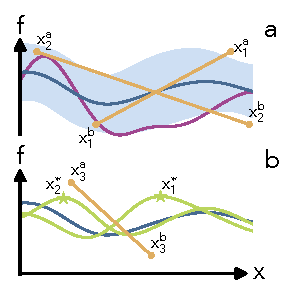
\includegraphics[width=\linewidth]{pes_plot}
    \caption{Learning from preferences. (a) Mean and standard deviation of
    $\prob{\vecf{f}[\tn{t}]|D_n}$ (blue) after two preferences queries (orange)
    from the true objective function (purple). (b) Mean of
    $\prob{\vecf{f}[\tn{t}]|D_n}$ (blue) and means of
    $\prob{\vecf{f}[\tn{t}]|D_n, x_m^*}$ (green) for two samples of $x_m^*$.
    PES-P queries a new comparison (orange) for which the preference is
    currently uncertain, but on average is certain after conditioning on all
    $x_m^*$.}\label{fig:pes_plot}
\end{marginfigure}

One such acquisition function is the expected improvement, which has been used
both in the context of preference feedback~\citep{eric2008active} and interval
scale feedback~\citep{jones1998efficient},
\begin{equation}
    \func{EI}{x} = (\mu^* - \mu(x))\Phi(d) + s(x)\phi(d),
    \label{eq:expected_improvement}
\end{equation}
where $d = (\mu^* - \mu(x))/s(x)$, $\mu^*$ is the mean of the current estimate
of the optimum, and $\mu(x)$ and $s(x)$ are the mean and standard deviation of
the objective of a new point $x$, respectively. As an alternative, for interval
scale feedback,~\citep{hennig2012entropy} and~\citep{hernandez2014predictive}
proposed acquisition functions that seek to reduce the uncertainty in the
distribution of objective function optima, measured in terms of the differential
entropy. For example, the Predictive Entropy Search acquisition
function~\citep{hernandez2014predictive} seeks a point $x$ that is expected to
reduce the entropy of the distribution of optima $x^*$ after observing its value
$y$,
\begin{align}
    \alpha_n \left(x \right) = \funcsb{H}{\prob{x^*|D_n}} 
        - \funcsb{E}[\prob{y|x, D_n}]{\funcsb{H}{\prob{x^*|y, x, D_n}}},
    \label{eq:pes_interval_scale}
\end{align}
where $\funcsb{H}{\prob{x}} = - \int \prob{x} \log \prob{x} \tn{d} x$
is the differential entropy. The authors of these methods have shown they can
outperform EI\@. 

\section{Bayesian Approach - Methods}
Our goal is to simultaneously address both the difficulty of defining objective
functions when an expert cannot demonstrate the desired robot behavior and the
expense of running experiments on hardware. To this end, we adapt the Predictive
Entropy Search acquisition function (\cref{eq:pes_interval_scale}) to the
preference learning case.

\subsection{Acquisition Function}
To obtain the optimal parameters $x^*$ with the smallest number of preference
queries, we solicit preferences that maximize the expected information gain
about the distribution of objective function optima $\mathrm{P}(x^*|D_n)$.
Adapting \cref{eq:pes_interval_scale} to preference feedback yields
\begin{fullwidth}
\begin{align}
    &\alpha_n \left(x^\tn{a}, x^\tn{b}\right) 
        = \funcsb{H}{\prob{x^*|D_n}} - \funcsb{E}[\prob{y|x^\tn{a},x^\tn{b},D_n}]
            {\funcsb{H}{\prob{x^*|y, x^\tn{a}, x^\tn{b}, D_n}}},
    \label{eq:acquisition_orig}
\end{align}
\end{fullwidth}
where $y$ is a binary random variable that represents the preference between
$x^\tn{a}$ and $x^\tn{b}$. The first term in this function is the current
entropy of objective function optima and the second term is the entropy of
optima after observing the preference $y$. As we have not yet observed the
preference, we take the second term in expectation over the two possible
preference outcomes.

As discussed in~\citep{hernandez2014predictive}, this acquisition function is
intractable to compute. However, following the approach used for the original
PES algorithm, we can rewrite~\cref{eq:acquisition_orig} in terms of the
entropies of the predictive distribution of the preference between $x^\tn{a}$
and $x^\tn{b}$,
\begin{fullwidth}
\begin{align}
    \alpha_n \left(x^\tn{a}, x^\tn{b} \right) &= 
        \funcsb{H}{\prob{y|x^\tn{a}, x^\tn{b}, D_n}}
            - \funcsb{E}[\prob{x^*|D_n}]{\funcsb{H}
            {\prob{y| x^*, x^\tn{a}, x^\tn{b}, D_n}}} \\
        &\approx \funcsb{H}{\prob{y|x^\tn{a}, x^\tn{b}, D_n}}
            - \frac{1}{M} \sum_{x_m^* \sim {\prob{x_m^*|D_n}}}^M 
            \hspace{-0.03in}\funcsb{H}{\prob{y| x_m^*, x^\tn{a},x^\tn{b},D_n}}.
        \label{eq:aq_approx}
\end{align}
\end{fullwidth}
This reformulation significantly improves computability. First, the new
acquisition function uses the entropies of probabilities of preferences, given
by~\cref{eq:p_pref}. Second, we now take the expectation over $\prob{x^*|D_n}$,
which we can perform by sampling $M$ functions from
$\prob{\vecf{f}[\tn{t}]|D_n}$ and optimizing each one to get $M$ samples of
$x^*$ (see Appendix for details). Finally, the second term no longer requires
conditioning the GP on every pair of $x^\tn{a}$ and $x^\tn{b}$ considered during
optimization of the acquisition function.  Instead, we only have to condition
the Gaussian process $M$ times on $(x_m^*, D_n)$.

For the experiments in~\cref{s:results} we choose $M = 12$, which allows us to
construct and optimize $\alpha_n(x^\tn{a}, x^\tn{b})$ in about five seconds,
which is fast enough for our prosthesis application. Although 12 samples of
$x^*$ is not enough to compute an accurate expectation over $\prob{x^*|D_n}$,
interpreting the algorithm as an example of active learning by disagreement may
explain why it still works well.  As shown in~\cref{fig:pes_plot}b, optimizing
the acquisition function chooses a pair $x^\tn{a}$ and $x^\tn{b}$ for which the
preference is currently uncertain, but certain on average after conditioning on
all $x_m^*$. The sampled $x_m^*$ do not necessarily agree on which point is
preferred; hence, after observing the preference, the algorithm can rule out
$x_m^*$ that made the model certain but wrong about the preference. This
intuition is similar to that provided by \citep{houlsby2012collaborative} for
Bayesian active learning by disagreement for GP classifiers.

\subsection[Conditioning the Gaussian Process on optima]{Conditioning the
Gaussian Process on $x^*$} The second term on the right side
of~\cref{eq:aq_approx} requires us to compute the distribution of the
preference given the location of the optimum,
\begin{fullwidth}
\begin{align}
&\prob{y| x_m^*, x^\tn{a}, x^\tn{b}, D_n} =
    \int \prob{x^\tn{a} \succ x^\tn{b} | \vecf{f}[\tn{t}], x_m^*, D_n} 
    \prob{\vecf{f}[\tn{t}] | x_m^*, D_n} \tn{d} \vecf{f}[\tn{t}].
    \label{eq:predic_pref_w_constraint}
\end{align}
\end{fullwidth}
It is not directly feasible to condition the predictive distribution on $x^*$,
so instead we turn to approximating this condition with three constraints (see
\hyperlink{sec:appendix}{appendix} for details):

C1: First we impose that $x^*$ is a local maximum by ensuring that the gradient
of $f(x^*)$ is zero and its Hessian is negative definite. We further simplify
the Hessian constraint to only require that the Hessian's off-diagonal elements
are zero and its diagonal elements are less than zero. We implement the gradient
and off-diagonal constraints by conditioning the prior, $\prob{\vecf{f}}$, on
derivative observations as outlined in~\citep{solak2003derivative}. To constrain
the diagonal elements of the Hessian, we amend the likelihood term in
\cref{eq:bayes_rule} by adding terms that penalize Hessians with positive
diagonal elements.

C2: Second, we try to ensure that $x^*$ is also a global maximum by enforcing
that $f(x^*)$ is greater than the function values of all training points sampled
so far. We impose this constraint by adding more preference relations into the
likelihood term in \cref{eq:bayes_rule} between $x^*$ and all training points.

C3: Finally, to further ensure that $f(x^*)$ is a global maximum, we require
that it is also larger than the function values of the two new test points,
$f(x^\tn{a})$ and $f(x^\tn{b})$. Whereas C2 ensures $f(x^*)$ exceeds function
values in areas explored so far, C3 ensures that $f(x^*)$ also exceeds function
values in unexplored regions. We approximate this constraint analytically by
conditioning on the single constraint $f(x^*) > (f(x^\tn{a}) + f(x^\tn{b}))/2$
using the method detailed in~\citep{xu2010estimation}.
\begin{algorithm}[t]
    \caption{Predictive Entropy Search with Preferences}
    \begin{algorithmic}[1]
        \Procedure{PES-P}{}
            \State{$D_n = \varnothing$}
            \For{$n \gets 0$ \textbf{to} $N-1$}\Comment{$N$ iterations}
            	\State{$F \gets \{\vecf{f}[m] \sim \prob{\vecf{f}[\tn{t}]| D_n} 
                    | m \in [1, M]\}$}
               	\State{$X^* \gets \{\arg \max_x \left(\vecf{f}[m] \right) 
                    | \vecf{f}[m] \in F \}$}
                \State{$(x_{n+1}^\tn{a}, x_{n+1}^\tn{b}) \gets \arg
                    \max_{(x^\tn{a}, x^\tn{b})} 
                    \funcil{\alpha}[n]{x^\tn{a},x^\tn{b};X^*}$}
                \State{$y_{n+1} \gets 
                    \textsc{QueryUserPref}(x_{n+1}^\tn{a}, x_{n+1}^\tn{b})$}
                \State{$D_{n+1}\hspace{-0.25em}\gets\hspace{-0.25em}
                    D_n \cup (x_{n+1}^\tn{a}, x_{n+1}^\tn{b}, y_{n+1})$}
            \EndFor{}
            \State{$\textbf{return} \ x^* \gets \arg \max_x
                \func{mode}{\prob{\vecf{f}[\tn{t}](x)| D_N}}$}
        \EndProcedure{}
        \Statex{}
        \Function{$\alpha_n$}{$x^\tn{a}, x^\tn{b}; X^*$}
            \Comment{acquisition function}
            \State{$h \gets \left\{\funcsb{H}{\prob{y|x^\tn{a}, x^\tn{b}, D_n, 
                \tn{C1}, \tn{C2}, \tn{C3}}} | x_m^* \in X^* \right\}$}
            \State{$\textbf{return} \ \funcsb{H}{\prob{y|x^\tn{a},x^\tn{b},D_n}} 
                - \func{mean}{h}$}
        \EndFunction{}
    \end{algorithmic}\label{alg:pesp}
\end{algorithm}

\subsection{Algorithm Summary}
With constraints C1 to C3, at each iteration we can efficiently compute the
acquisition function, \cref{eq:aq_approx}. We summarize the resulting Predictive
Entropy Search with Preferences (PES-P) algorithm as follows (\cref{alg:pesp}):
At each iteration $n$, first, the algorithm samples $M$ objective functions from
the current distribution, $\prob{\vecf{f}[\tn{t}]|D_n}$, and optimizes each one
to generate $M$ samples of $x^*$ (lines 4 and 5).  Next, using the set of
sampled optimums $X^*$, we maximize the acquisition function to obtain the next
two points to present to the user $x_{n+1}^\tn{a}$ and $x_{n+1}^\tn{b}$ (lines 6
and 12--15). Note: we can precompute the effect of C1 and C2 before evaluating
$\funcil{\alpha}[n]{x^\tn{a}, x^\tn{b}}$ as these two constraints do not depend
on $x_{n+1}^\tn{a}$ and $x_{n+1}^\tn{b}$. On the other hand, C3 depends directly
on $x_{n+1}^\tn{a}$ and $x_{n+1}^\tn{b}$ and therefore is computed within the
acquisition function for every pair of points considered during the optimization
of $\funcil{\alpha}[n]{x^\tn{a}, x^\tn{b}}$. We then query the user to obtain
their preference $y_{n+1}$ between these two points and add it to the dataset of
preferences (lines 7 and 8). Finally, at the end of the $N$ iterations of the
algorithm, we return the optimum $x^*$ of the most likely function,
$\func{mode}{\prob{\vecf{f}[\tn{t}](x)| D_N}}$, which is equal to the posterior
mean function in the Gaussian process case (line 10). While it may be more
correct to return $\func{mode}{\prob{x^*|D_N}}$, we do not do this as the PES
algorithm seeks to avoid approximating this distribution.

\section{Bayesian Approach Results}\label{s:results}
We test the ability of PES-P to solve optimization problems in four cases with
increasing realism from the optimization of randomly generated objective
functions drawn from a GP, to the tuning of feedback gains of random linear
systems and a neuromuscular walking model, to the optimization of control
parameters for a powered transfemoral prosthesis given real user feedback. In
all four cases, we compare the performance of the proposed algorithm to the
expected improvement criterion (EI) (\cref{eq:expected_improvement}) and random
sampling via Latin hypercubes (LH)\sidenote[][2.25in]{LH sampling divides the
parameter space into ${(2N)}^D$ hypercubes, where $D$ is the dimensionality of
the space.  $2N$ samples are placed such that each hypercube has at most one
sample and there is at most one filled hypercube along any row of hypercubes
when viewed along any direction.  This method ensures that the samples are
roughly uniformly distributed in the entire space. At each iteration we choose
two of these samples to query users.}~\citep{mckay2000comparison}. For the three
simulated cases, we show results over 20 trials and measure performance in terms
of the immediate regret, defined as $IR = |f(\tilde x_n^*) - f(x^*)|$, versus
the number iterations.  Here, $f(\tilde x_n^*)$ is the objective value of the
current estimate of the optimum at this iteration, $f(x^*)$ is the value of the
true optimum, and an iteration consists of a single preference query between two
points.  Additionally, we also check the statistical significance of the
reduction in IR obtained by PES-P compared to both EI and LH via two-sided
Mann-Whitney $U$ tests $(p < 0.05)$.

\begin{figure*}[t!]
    \centering
    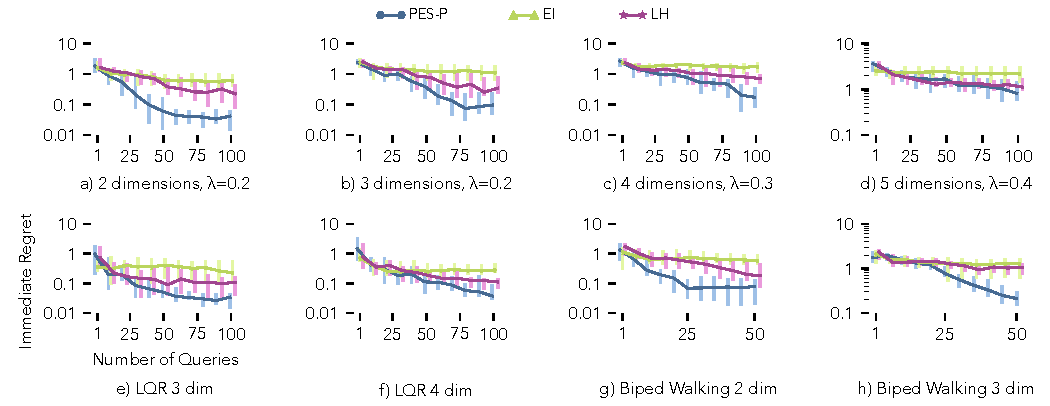
\includegraphics[width=\textwidth]{pes_results}
    \caption{Performance of predictive entropy search with preferences (PES-P),
    expected improvement (EI), and Latin hypercube random sampling (LH) for
    optimizing random objective functions sampled from a GP (a-d), and tuning
    feedback control parameters of random linear systems (e-f) and a biped
    walking model (g-h). Shown are the median and interquartile range over 20
    trials of the immediate regret (IR) against the number of preference
    queries. Black stars indicate iterations for which PES-P achieves
    statistically significant stochastic reductions in IR compared to both EI
    and LH according to two-sided Mann-Whitney $U$ tests $(p <
    0.05)$.}\label{fig:y_err_sim}
\end{figure*}

\subsection{Optimizing Randomly Generated Objective Functions}

To avoid inducing bias by hand-engineering test functions, we first evaluate the
algorithm on random synthetic objective functions. We generate objective
functions on the domain $x \in {[-1, 1]}^D$ by sampling a vector of 500 function
values from a GP prior with a quadratic mean, $\mu(x) = - x^\tn{T} x$, and
isometric squared exponential covariance $\funcil{k}{x_i,x_j} = \exp
\left(\frac{-1}{2 \lambda} x_i^T x_j \right)$. We use a quadratic mean function
to bias the function distribution away from those that have their optimum on a
boundary of the domain, as these functions are easier to optimize. We continue
to generate the rest of the function as it is optimized by conditioning the GP
on the 500 seed values and all function values sampled during the optimization.
We assume the mean of the final function distribution is the true objective
function. To simulate more realistic situations, we provide the algorithms with
noisy preferences from the sampled function values ($\sigma^2 = 0.1$).

Figures~\ref{fig:y_err_sim}a-d show the immediate regret for two to five
dimensional problems with $\lambda$, the length scale of the kernel, scaling
from 0.1 to 0.4 as the dimensionality of the problem increases. On two to four
dimensional problems, PES-P outperforms EI and LH by achieving statistically
significant reductions in IR\@. However, as the dimensionality increases, it
takes more iterations for this advantage to become apparent. In the five
dimensional case, there is no significant difference between PES-P and LH,
likely due to $M=12$ samples of $x_m^*$ being insufficient and the difficulty of
accurately sampling $x_m^*$ in higher dimensions.

\subsection{Tuning Controllers for Random Linear Systems}
Next, we test the ability of PES-P to optimize simple control systems by
optimizing the feedback gains $K$ for $D$-dimensional single-input linear
systems $\dot{\xi} = A \xi + Bu$ with feedback $u = K \xi$. We sample the
elements of the $A$ matrix from the standard normal distribution while $B =
{[0_{1 \times (D-1)}, 1]}^\tn{T}$. We assume a quadratic instantaneous cost
resulting in the objective function
\begin{equation}
    f(K) = - \int_0^{t_f} \xi_K^\tn{T}(t) (Q + K^T R K) \xi_K(t) dt,
\end{equation}
where $\xi_K(t)$ is the evolution of the state under the control policy $K$ and
a fixed initial condition $\xi_0$, $Q = I_{D \times D}$ and $R = 1$. To obtain a
finite search domain, we find the stable range of parameters by varying the
elements of the true optimal control parameters $K^*$ one at a time while
keeping other elements constant. We scale and shift this region to map to the
domain ${[-1, 1]}^D$. Finally, we use the Automatic Relevance Determination
Gaussian Kernel and optimize the hyperparameters at each iteration by maximizing
the posterior probability of the hyperparameters under a gamma
hyperprior~\citep{chu2005preference,
williams2006gaussian}. In order to apply a consistent noisy preference model
$(\sigma^2 = 0.1)$ across all sampled systems, we transform all objective values
by first mapping them through $-\log(-f(K))$ and then shifting and scaling the
values by the mean and range of the values of $10^D$ randomly sampled
controllers. 

Figures~\ref{fig:y_err_sim}e and~\ref{fig:y_err_sim}f show the resulting
optimization performance on three and four dimensional systems. In the 3
dimensional case, PES-P achieves a lower median IR than LH after 30 iterations.
This difference becomes significant after 60 iterations. In the 4 dimensional
case, PES-P significantly outperforms LH after 50 iterations, but the
significance of this improvement is sporadic as the iterations continue. A
possible reason for the reduced performance difference between PES-P and LH in
the LQR problem as compared to the random objective function problems is the
existence of hard-to-optimize flat regions in the LQR objective functions. This
suggests that PES-P may be more well suited for problems that have clear
optimum.
\subsection{Tuning Control Parameters of a Walking Model
    }\label{sec:sim_neuro}
In the third case, we test the ability of PES-P to optimize the feedback gains
for a neuromuscular model of walking~\citep{thatte2016toward}, a system with a
complex non-linear controller addressing the specific application domain of
human locomotion. We perform two and three dimensional optimizations, in which
we tune the feedback gains for a subset of the model's muscle actuators.  We use
the negative cost of transport plus the distance walked over a 20 second time
span as the objective function. As in the previous linear systems example, we
obtain noisy preferences between parameters and optimize the hyperparameters at
every iteration.

Figures~\ref{fig:y_err_sim}g and~\ref{fig:y_err_sim}h show the performance of
PES-P, EI, and LH\@. In this example, PES-P achieves a significant reduction in
IR in just 10 iterations in the 2-dimensional case and in 25 iterations in the 3
dimensional case.  Furthermore, in the 3D case the PES-P's median solution is
approximately 10 times better than those found by EI or LH\@. 

\section{Bayesian Approach Discussion}\label{sec:bayes_discussion}
We presented a new optimization algorithm (PES-P) that extends Predictive
Entropy Search to preference feedback. The algorithm addresses two key problems
frequently encountered in system optimization. First, it circumvents the often
difficult process of parameterizing and learning an objective function by
directly querying users for preferences between pairs of parameters. Second, the
algorithm minimizes the required number of experiments by employing Bayesian
optimization techniques that ensure the queries maximize the information gained
about the location of the optimum. Moreover, unlike previous approaches for
preference learning on robotic systems~\citep{wilson2012bayesian,
jain2013learning}, PES-P does not require a model of the system.

Our experiments show that the proposed algorithm outperforms baseline
algorithms. In most of the experiments, PES-P found optima that achieved higher
objective values than those found by the expected improvement method (EI) or by
random comparisons via Latin hypercubes (LH) (\cref{fig:y_err_sim}). The reason
why PES-P outperformed EI is likely due to the former's explicit consideration
of how the limited, noisy information obtained from a preference query will
affect the knowledge about potential objective function optima. The acquisition
function (\cref{eq:acquisition_orig}) recognizes that preferences become more
uncertain the closer two sample points are to each other. EI, on the other hand,
does not reason about noisy preferences and, instead, still assumes it can
sample values (\cref{eq:expected_improvement}). Consequently, EI ignores the
distance between sample points, which often leads to a greedy strategy that
solicits preferences between adjacent points. While this strategy can resemble
gradient ascent with convergence to local optima in a noise-free optimization,
it often failed in our experiments characterized by noisy observations. Note,
however, that such limitations were not observed by Brochu and
colleagues~\citep{eric2008active}, who successfully used EI with preferences to
optimize parameters for a graphics application, possibly because the associated
visual task produced less noisy responses than did our simulations. 

However, a major drawback of the proposed PES-P approach is its limited ability
to scale to problems of sufficient dimensionality. As shown in
\cref{fig:y_err_sim}d PES-P provides little benefit over random sampling on 5D
problems. In contrast, to optimize the neuromuscular model control proposed in
\cref{sec:nm_control_prosthesis} we need to be able to solve problems with
dozens of dimensions. Therefore, in the next half of this chapter, we explore an
alternative approach, that frames prosthesis optimization as a dueling bandits
problem \citep{yue2012k}.

\section{Bandit Approach - Introduction} 

There is a clear trend in research and recent commercial products towards
robotic prostheses that promise to ameliorate the gait deficiencies imposed by
prevailing mechanically-passive devices. With the robotization of prostheses,
clinicians can now tune a large number of control parameters in order to
maximize the performance of these devices for each user.

Given the variability in human gait patterns, it is important to tailor these
gait policies for specific users.  Recently, \citet{zhang2017human} demonstrated
this by optimizing an ankle exoskeleton's torque trajectory for specific users.
The authors found that optimized torque trajectories could reduce metabolic
energy consumption beyond that provided by a generic assistance strategy.

Others have investigated optimization methods for prostheses specifically. For
example, \citet{huang2016cyber} propose a cyber expert system that uses
pre-defined rules to modify impedance control parameters in order to improve the
trajectory-tracking performance of a powered knee prosthesis. This approach was
later improved by using adaptive reinforcement learning to circumvent
predefining the tuning rules \citep{wen2016adaptive}. 

A drawback of these previously proposed methods are their reliance on numeric
optimization criteria, such as metabolic energy or trajectory tracking
performance. It is unclear if optimizing prostheses to follow a specific
trajectory will result in a positive outcome given the asymmetries in actuation,
kinematics, and inertia induced by an amputation and wearing a prosthesis.
Moreover, myopic optimization of a single aspect of gait may neglect other
characteristics that are often subjective such as comfort and confidence.
Therefore, in this work, we utilize subjective preferences between pairs of
policy parameters in order to achieve a more holistic approach to prosthesis
optimization.

A second difficulty for existing methods is tackling the high dimensional,
constrained optimization problem imposed by multi-joint assistive devices such
as transfemoral prostheses. Previously published impedance control strategies
for transfemoral prostheses have roughly 30 tunable parameters for a given gait
condition, such as walking at a specific speed. \citet{sup2011upslope} show that
these parameters also vary with alternative conditions such as incline.
Therefore, these kinds of parameterized policies could require on the order of
100 parameters to deal with a range of situations. Previous work has attempted
to reduce the number of parameters via heuristic rules that tie impedance
parameters to other states of the prosthesis such as joint angles
\citep{simon2014configuring}.  However, it is not obvious how to translate these
heuristics to other control strategies, such as neuromuscular control
\citep{thatte2016toward}, which models muscles and neural reflexes, or
phase-based control \citep{quintero2016preliminary}, which follows knee and
ankle trajectories parameterized as functions of hip angle and hip angle
integral.

To deal with high-dimensional parameter selection for prostheses, many have
turned to offline optimization of control parameters \citet{markowitz2011speed}
use data from a height-and weight-matched intact subject to obtain
speed-adaptive neuromuscular control parameters for a transtibial amputee's
prosthesis and \citet{aghasadeghi2013learning} use an invariant gait
representation to model an amputee's gait and find the appropriate impedance
control parameters. In these approaches however, it is unclear how well the
resultant parameters suit the subject when executed on actual hardware.

In this paper, we tackle these issues by framing prosthesis optimization as a
dueling bandits problem \citep{yue2012k}. The resulting approach utilizes the
subject's preferences to include subjective user feedback in the tuning process.
The method deals with high dimensional optimization problems by incorporating
domain knowledge in the form of an offline optimization step. We show that this
method produces a library of parameters from which different users prefer
different options and for which preferred controllers tend to follow human gait
trends. Moreover, we explore further utilizing the offline optimization to help
the controllers generalize to speeds that were not included during the online
optimization process.

\section{Bandit Approach Methods}\label{sec:bandit_methods}

In this study, we use the transfemoral prosthesis presented in
\cref{sec:pros_design} and the neuromuscular prosthesis control described in
\cref{sec:nm_control_prosthesis}. 

\subsection{Optimization method}\label{sec:bandit_optimization}

To optimize the control parameters of this neuromuscular transfemoral prosthesis
control for specific users, we frame the task as a $K$-armed dueling bandits
problem \citep{yue2012k}. In this formalism, at each iteration $t \in [1,\ldots
T]$ of the optimization, an algorithm chooses two options, referred to as
bandits, out of the set of $K$ possibilities, so as to minimize the total
cumulated regret over the iterations. The cumulated regret is defined as
\begin{align}
    R(T) = \zeta^* T - \frac{1}{2} \sum_{t=1}^T \funcsb{E}{\zeta_{1t} + \zeta_{2t}}
\end{align}
where $\zeta^*$, $\zeta_{1t}$, and $\zeta_{2t}$, are the values of the optimal
bandit and first and second bandits chosen on iteration $t$ respectively. To
minimize $R(T)$, algorithms must effectively trade of exploration of all bandits
to gain confidence in their values and exploitation of the best bandit so as to
not incur regret.

In a dueling bandits problem, we do not observe numeric rewards directly.
Rather, we observe if an oracle prefers the first bandit to the second.  Because
we never directly observe numeric values, algorithms for this problem use
alternative notions of value. In this work, we utilize the Double Thompson
sampling method \citep{wu2016double}, which achieves state-of-the-art regret on
several datasets. This method defines a bandit's value as its Copeland Score:
the number of other options that a bandit defeats on average.

Key to employing this method for prosthesis optimization is offline generation
of parameter sets for which we are likely to obtain reasonable gaits for
different subjects. This task can be viewed as sampling from the set of
parameters that produce gait patterns consistent with human locomotion. In this
work, we explore generating this set of controllers using a recently published
gait data set that includes kinematics and kinetics for individual subjects
walking at three different speeds, \unitfrac[0.8, 1.2, and 1.6]{m}{s}
\citep{moore2015elaborate}.  For each subject in this dataset, we use the
Covariance Matrix Adaptation Strategy \citep{hansen2006cma} to find
neuromuscular model parameters $\Gamma$ that reproduce the subject's
body-weight-normalized knee and ankle joint torques $\tau_\tn{h} =
[\tau_\tn{h}^\tn{k},\tau_\tn{h}^\tn{a}]^T$ given the subject's hip, knee, and
ankle angle trajectories $\theta_\tn{h} =
[\theta_\tn{h}^\tn{h},\theta_\tn{h}^\tn{k},\theta_\tn{h}^\tn{a}]^T$.
Specifically, we solve
\begin{align}
    \Gamma &= \argmin_\Gamma \left(\tau_\tn{h} - \tau_\tn{nm} \right)^T
    \left(\tau_\tn{h} - \tau_\tn{nm} \right) + \alpha \xi_\tn{nm}^T \xi_\tn{nm}
\end{align}
where $(\tau_\tn{nm}, \xi_\tn{nm}) = \func{neuro}[\Gamma][]{\theta_\tn{h}}$ are
the torques and muscle activations generated by the neuromuscular model given
the human joint angle trajectories and model parameters. $\alpha = 0.01$ is a
small constant we use to help regularize the solutions.

\begin{margintable}[1in]    
    \centering
    \small
    \begin{tabular}{ll|l}
        \multicolumn{2}{c|}{Speed-Independent} & Speed- \\
                                         &     & Dependent \\
        \midrule
        $F_\tn{max}^\tn{ham}$            & ham $\phi_0^\tn{hip}$   & $^{F+}G_\tn{ham}^\tn{ham}$   \\
        $F_\tn{max}^\tn{vas}$            & ham $\phi_0^\tn{knee}$  & $^{F+}G_\tn{vas}^\tn{vas}$   \\
        $F_\tn{max}^\tn{bfsh}$           & vas $\phi_0$            & $^{F+}G_\tn{gas}^\tn{gas}$   \\
        $F_\tn{max}^\tn{gas}$            & bfsh $\phi_0$           & $^{F+}G_\tn{sol}^\tn{sol}$   \\
        $F_\tn{max}^\tn{sol}$            & gas $\phi_0^\tn{knee}$  & $^{F-}G_\tn{sol}^\tn{ta}$    \\
        $F_\tn{max}^\tn{ta}$             & gas $\phi_0^\tn{ankle}$ & $^{L+}G_\tn{bfsh}^\tn{bfsh}$ \\
        $^\tn{off}l_\tn{bfsh}^\tn{bfsh}$ & sol $\phi_0$            & $^{L-}G_\tn{bfsh}^\tn{vas}$  \\
        $^\tn{off}l_\tn{bfsh}^\tn{vas}$  & ta  $\phi_0$            & $^{L+}G_\tn{ta}^\tn{ta}$     \\
        $^\tn{off}l_\tn{ta}^\tn{ta}$     & $S_0^\tn{vas}$          & \\
                                         & $S_0^\tn{ham}$          & \\
    \end{tabular}
    \caption[Parameters optimized to generate parameter sets for dueling bandits
    optimization]{Optimized parameters, $\Gamma$. Speed-independent parameters
    use a single value for all speeds, while speed dependent parameters have
    distinct values for \unitfrac[0.8, 1.2, and 1.6]{m}{s} gaits. Consequently,
    in total we optimize 43 parameters. $F_\tn{max}$ refers to a muscle's maximum
    isometric force, $\phi_0$ is a parameter used for muscle moment arm
    calculations, and $S_0$ is a muscle's pre-stimulation.}\label{tab:params}
\end{margintable}
\Cref{tab:params} shows the parameters we optimize during this process.  For
each parameter in the Speed-Independent category, we look for a single value to
use across all speeds. For parameters in the Speed-Dependent category we search
for three different values, one for each gait speed in the dataset
(\unitfrac[0.8, 1.2, and 1.6]{m}{s}). The parameters we choose to optimize
include the isometric force and feedback gains for each muscle, which are
closely related to the effective stiffness of the
joint~\citep{geyer2003positive}, muscle prestimulations, which are related to
the stride energy~\citep{geyer2003positive}, and the muscle reference angles, to
help deal with the kinematic variability between
subjects~\citep{geyer2010muscle}.

From the dataset provided by \citet{moore2015elaborate}, which contains samples
for twelve subjects, we were able to extract nine parameter sets. (One subject's
torque data is corrupted and two subjects' data resulted in an overly flexed
knee when used on the prosthesis.) \Cref{fig:nm_fit} shows an example of two
subjects' torque patterns shown in red. We see that there are significant
differences between the two subjects in terms of both timing and magnitude of
torque. In green, we see that after optimizing the neuromuscular model for each
subject, it is able to capture both gait patterns. 

We can quantify the quality of the model fit to the data by computing the root
mean squared (RMS) error between the model's predicted torques and the actual
torques. Over the nine parameter sets we achieve a median RMS knee torque error
of 35\% of the RMS human knee torque, and a median RMS ankle torque error of
15\% of the RMS human ankle torque. Much of the error in the knee torque
prediction occurs right after heel strike, where the model typically predicts
near-zero torque. In future work we plan to adapt the model to produce more knee
flexion torque at heel strike, which should significantly reduce the model
error.

To compensate for kinematic differences between the prosthesis and the training
data, before sending prosthesis joint angles to the neuromuscular control, we
add constant bias angles to the joint encoder readings so that at joint $j$,
\begin{align}
    \theta_\tn{model}^j = \theta_\tn{encoder}^j + \theta_0^j.
    \label{eq:bias_param}
\end{align}
We hand-tune these bias parameters for each bandit and subject to ensure the
bandits work as well as possible.
 
\begin{figure}[htb]
    \centering 
    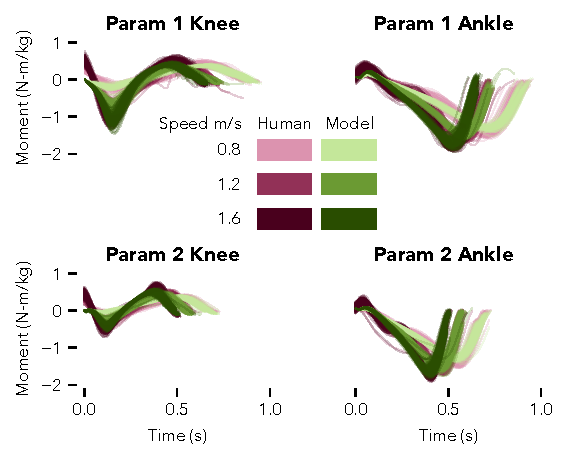
\includegraphics[width = \columnwidth]{nm_fit_w_legend.pdf}
    \caption[Results of offline optimization to fits neuromuscular model to
    intact-subject gait data at different speeds]{Results of the offline
    optimization that fits the neuromuscular model to intact-subject gait data.
    Shown are the knee and ankle torques for two different subjects.  These
    plots show there can be significant inter-subject gait
    variability.}\label{fig:nm_fit}
\end{figure}

\subsection{Experiment Procedure}
In our experiment, we test the ability of our offline optimization approach to
generate controllers that are suited to different subjects and to produce
kinematics and kinetics similar to those of intact subjects. We further test the
effectiveness of using offline optimizations to help improve the ability of the
control to generalize to speeds different than those experienced during the
online optimization.

After providing informed consent to a protocol approved by the Carnegie Mellon
University Internal Review Board, five non-amputee subjects (four male, one
female, average mass = \unit[68.8]{kg} std \unit[11.17]{kg}) donned the
prosthesis via the able-bodied adaptor shown in \cref{fig:prosthesis_actual}. On
the contralateral leg, subjects wore a lift shoe, the height of which we
adjusted to ensure subjects' hips were even when standing.

Subjects participated in a three day study. On the first day, subjects
acquainted themselves with the prosthesis for roughly 2 hours. By the end of
this period, all subjects were able to walk (while holding hand rails)
consistently without tripping on a set of hand-tuned parameters at a speed of up
to \unitfrac[1.2]{m}{s}. On the second day, the first 15 minutes consisted of
hand-tuning the bias angles for each parameter set (\cref{eq:bias_param}) to
allow the subject to achieve adequate ankle and knee flexion for as many
parameters as possible. Then, we performed the dueling bandits optimization for
50 iterations, which required approximately thirty minutes of walking at
\unit[0.8]{m/s}. Each iteration consisted of roughly ten seconds of walking on
each parameter, after which the subject indicated their preference. If subjects
were unsure of their decision they could walk with both parameter sets multiple
times. If their uncertainty persisted, the experimenter chose the parameter set
that produced angles and torques more aligned with human data.  If the
experimenter also had no preference, a random number generator selected the
winner. We chose to perform fifty iterations, as pilot testing suggested this
was sufficient for the algorithm to begin comparing the optimal parameter set to
itself, indicating a high level of confidence in the optimum.

On the third day, subjects walked with their preferred parameters at
\unitfrac[0.8, 1.0, 1.2, 1.4, and 1.6]{m}{s}. For each speed, we tested both the
appropriate speed-dependent parameters and those designed for
\unitfrac[0.8]{m}{s}. To obtain parameters for \unitfrac[1.0 and 1.4]{m}{s} we
performed linear interpolation between the adjacent parameters.  Finally, we
recorded the subject's gait at \unitfrac[0.8]{m}{s} for all non-preferred
parameter sets and the hand-tuned parameters used on the first day. 

\section{Bandit Approach Results} 

\subsection{Copeland Scores}

The five subjects in the study preferred four different parameter sets out of
the nine parameter sets they could choose from, thereby demonstrating that the
offline optimization approach can generate parameters that suit different users.
\Cref{fig:copeland} shows the total Copeland score achieved by each parameter
set across all five subjects. From this chart, we can see it is possible, as in
the case of parameter set 6, that a controller receives high scores from some
users while receiving a score of zero from other users. This illustrates the
importance of tailoring prostheses to individual users. Some parameters such as
parameters 1, 4, and 8, achieved consistently low scores across all users. It
may be possible for us to remove these parameters from future studies. However,
more subjects would be needed before making such a determination as parameter
set four received a relatively high score from subject five.

\begin{figure}[b]
    \centering
    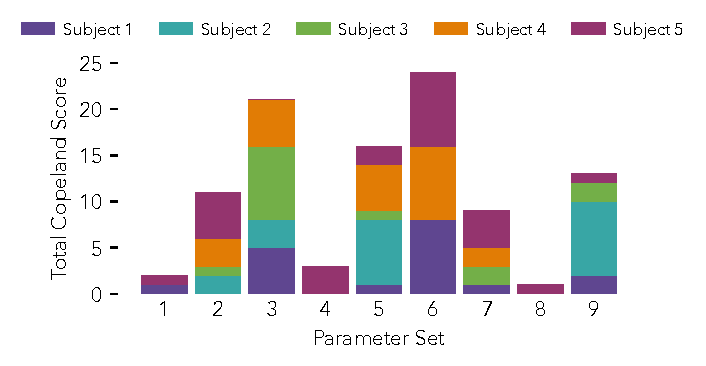
\includegraphics[width=\columnwidth]{copeland_scores_new}
    \caption{Total Copeland score achieved by each parameter set across all five
    subjects.}\label{fig:copeland}
\end{figure}

\begin{figure}[t]
    \centering
    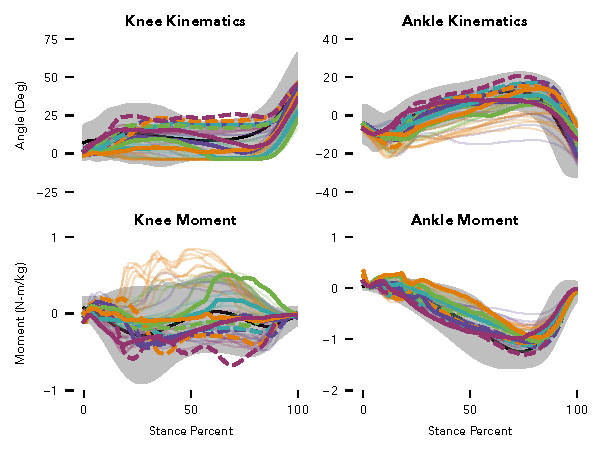
\includegraphics[width=\columnwidth]{kin_all_arms}
    \caption[Median angles and moments for all parameter sets for all
    subjects.]{Median angles and moments at \unitfrac[0.8]{m}{s} for all
    parameter sets for all subjects. Thicker weight solid lines indicate each
    subject's gait with their preferred parameters. Dashed lines indicate gait
    with hand-tuned parameters. The grey shaded regions show the mean and three
    sigma intact subject gait data (from the extra slow walking data in
    \citep{bovi2011multiple}).}\label{fig:kin_all_arms} 
\end{figure}

\subsection{Kinematics and Kinetics at \unitfrac[0.8]{m}{s}}
\Cref{fig:kin_all_arms} shows the ankle and knee kinematics achieved by all
subjects on all parameters at \unitfrac[0.8]{m}{s}. The thicker solid lines
indicate the gait data produced by subjects' preferred parameters and the dashed
lines indicate the gait data produced by the hand-tuned parameters. We see that
subject gait with both their preferred parameters and hand-tuned parameters
follow similar trends to intact gait data~\citep{bovi2011multiple}, whose mean
and three sigma variance is shown as the blue shaded region. However, all
subjects preferred the optimized parameters to the hand-tuned set. 

Just as in the intact data, there is significant variation in subjects'
preferred gait characteristics, which reinforces the idea that targeting a
specific kinematic or kinetic pattern may not be ideal for all users. This seems
to be especially true of the knee joint moment, where there are significant
differences in the amount of knee extension torque in early stance and flexion
torque in late stance among users. 

\begin{comment}
We found that most subjects produced relatively little ankle dorsiflexion as
they walked. Consequently, for most subjects the neuromuscular model control
produced less ankle plantarflexion torque than is average for able-bodied
subjects.  We believe the low level of ankle dorsiflexion was caused by the
relatively short foot of the prosthesis, which we plan to rectify for future
experiments. However, this effect also betrays a potential weakness of the
approach: optimizing to match able-bodied kinetics given able-bodied kinematics
may not be able to rectify some types of discrepancies between the human and
the prosthesis.
\end{comment}

\subsection{Control Performance at Higher Gait Speeds}
\begin{figure}
    \centering
    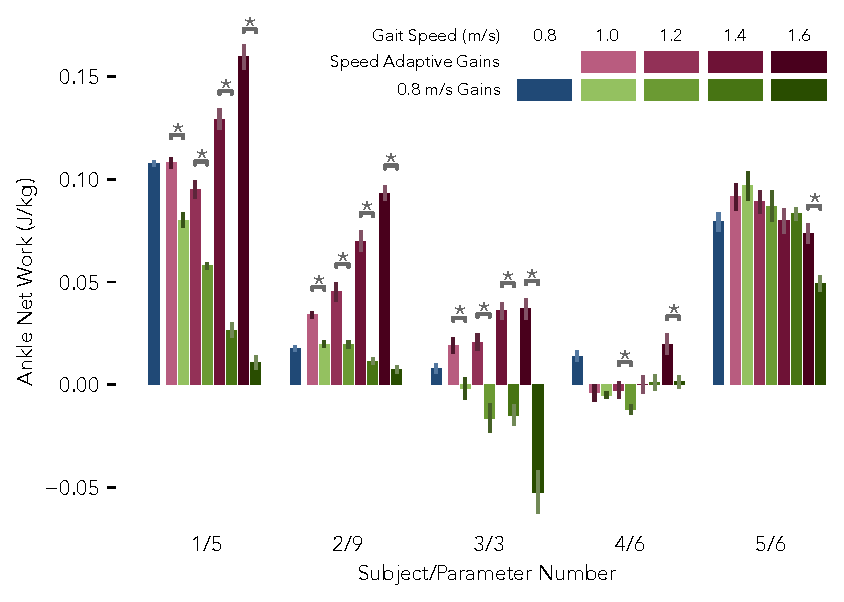
\includegraphics[width=\columnwidth]{net_work_vs_speed_new_annotated}
    \caption[Average net ankle work for each subject at each speed]{Average net
    ankle work for each subject at each speed. Purple bars indicate trials where
    speed-adaptive gains were used whereas green bars indicate trials performed
    with the gains for \unitfrac[0.8]{m}{s}. Stars indicate statistically
    significant differences between the work produced by the speed adaptive
    gains and that produced by the \unitfrac[0.8]{m}{s} gains $(p <
    0.05)$.}\label{fig:net_work_vs_speed}
\end{figure}

\Cref{fig:net_work_vs_speed} shows the average net ankle work\footnote{The area
within the torque versus angle plot of the ankle over a stride.} produced by the
control strategy at speeds ranging from \unitfrac[0.8 to 1.6]{m}{s}. Data from
subjects 1, 2, and 3, who chose parameter sets 5, 9, and 3 respectively, show a
clear downwards trend in ankle work as speed increases when using a constant set
of gains. On the other hand, with the adaptive gains, as speed increases ankle
work increases, mimicking the behavior of the biological ankle
\citep{herr2012bionic}. All three of these subjects preferred the behavior of
the adapted parameters to the parameters for \unitfrac[0.8]{m}{s} when walking
at \unitfrac[1.4 and 1.6]{m}{s}.

Subjects 4 and 5 both chose parameter set six and show no clear trend in ankle
work as speed increases. For this parameter set, the speed adapted gains only
increased ankle work significantly over baseline at \unitfrac[1.6]{m}{s} for
both subjects. Additionally, these two subjects indicated no trend in
preference between the adapted and unadapted parameters at the higher speeds.
These two subjects produced different amounts of net work despite using the same
parameter set. This is likely due to kinematic differences between the subjects
as well as differently tuned bias settings for the ankle joint.

From this result we can conclude that the offline optimization approach can
produce improved responses at speeds other than that at which we conduct the
online optimization, but that the improvement needs to be confirmed on a
per-parameter basis. It is not currently clear why parameter set six does not
exhibit increasing ankle work as speed increases as the underpinning human data
for this parameter set does indeed exhibit the desired trend. The issue could
possibly lie with the structure of the high level control or with local minimums
obtained by the CMA-ES method. 

\section{Bandit Approach Discussion}\label{sec:bandit_discussion}

We present a new approach for online optimization of lower limb assistive
devices that uses preference feedback to incorporate the user's subjective
assessment of device behavior. The method tackles high dimensional tuning
problems by incorporating domain knowledge via an offline optimization step that
utilizes kinetic and kinematic data from intact subjects to obtain a library of
policy parameters. We find that the five subjects who completed our experiment
preferred four different parameter sets from this library. The resulting gait
patterns resembled intact human gait data and were preferred to hand-tuned
parameters, confirming that the method can generate parameters suited for
different subjects.

A result of the offline optimization we use is that the method is largely
agnostic to the number of tunable parameters. Consequently, we were able to
additionally optimize neuromuscular model parameters for different speeds.  Our
experimental results show that these parameters improved the ankle work
characteristics and user preferences as speed increased for three out of four
tested parameter sets. 

Previous works such as \citet{eilenberg2010control} and
\citet{markowitz2011speed} have demonstrated control of powered ankle prostheses
via neuromuscular models of muscles and reflexes. This paper extends that work,
as it presents the first instance of neuromuscular control on a powered knee and
ankle prosthesis.

Due to the ability of the method to handle problems of arbitrary dimensionality
given sufficient computational resources, it may be used to tune many types of
control strategies. For example, one could use the approach to optimize the
phase variable control strategy, in which the prosthesis follows predefined knee
and ankle trajectories parameterized as functions of hip angle and hip angle
integral~\citep{quintero2016preliminary}. In this case, each bandit would
provide a different knee and ankle trajectory.  Importantly, the ability of this
method to optimize various types of controllers may help researchers compare
control strategies fairly, as we do in \cref{sec:nm_vs_imp}.

It is probable that the parameter library we obtained in this work can be
further improved. We propose two directions for further investigation: First, it
may be possible to improve the library by obtaining a larger set of gait data
and then using clustering algorithms to arrive at a reduced set of canonical
gaits. \citet{vardaxis1998classification} apply a similar idea to to EMG data to
cluster gaits into five major styles. With a library derived from canonical
gaits, we may cover the parameter space more evenly. A second approach is to use
biomechanical measurements from the amputee, such as segment lengths and
measured peak joint torques, to obtain probability distributions for the
neuromuscular model parameters. We could then compose the parameter library by
sampling parameters from the distributions and performing rigid body simulations
of the amputee and prosthesis system.

The optimization approach we have presented may have considerable practical
value for commercial prostheses as well. Because it uses preference feedback,
users of an assistive device can easily provide feedback via smartphones or
wearable devices. Moreover, the dueling bandit algorithm is well suited to
lifelong learning. Since the algorithm seeks to minimize regret, we can ensure
its exploration is only as obtrusive as necessary. 

The study we presented has several limitations. First, we only had five subjects
complete the study. Ideally, we would have more subjects than the number of
parameter sets so we could determine if any parameters are never preferred or if
any group is not currently well represented by the current set of parameters.
Also, we should confirm that the proposed optimization framework provides
suitable control parameters for amputees wearing this prosthesis.

\hypertarget{sec:appendix}{\section*{Bayesian Approach Appendix}}

To obtain $X^*$ (line 5,~\cref{alg:pesp}), we sample $M$ functions from the
posterior by approximating $\prob{\vecf{f}[\tn{t}]|D_n}$ using Bayesian linear
regression with Fourier features (as outlined in~\citep{hernandez2014predictive})
and sampling $M$ feature weight vectors. As the Fourier features have analytic
derivatives, we can optimize each linear function using a second order method
with multiple restarts.

We approximate conditioning the predictive distribution on $x^*$ via three
constraints: 
\begin{description} 
    \item[C1] $x^*$ is a local maximum. $\nabla f|_{x^*} = 0$ and the
    Hessian of the objective function is negative definite by imposing
    $\func{diag}{\nabla \nabla f|_{x^*}} < 0$ and $\func{upper}{\nabla
    \nabla f|_{x^*}} = 0$. We group $\nabla f|_{x^*} = 0$ and
    $\func{upper}{\nabla \nabla f|_{x^*}} = 0$ into constraint C1.1 and
    $\func{diag}{\nabla \nabla f|_{x^*}} < 0$ into constraint C1.2.

    \item[C2] $x^*$ is preferred to current training points, $f(x^*) >
    f(x_k^\tn{a}) \textrm{ and }  f(x^*) > f(x_k^\tn{b}), \ \forall k \in [1,
    n]$.

    \item[C3] $x^*$ is preferred to new training points, $f(x^*) >
    f(x_{n+1}^\tn{a})$ and $f(x^*) > f(x_{n+1}^\tn{b})$.  
\end{description}

We precompute the effects of contraints C1 and C2 before evaluation of
$\funcil{\alpha}[n]{x^\tn{a}, x^\tn{b}}$. To impose C1 and C2, we first divide
their components into two groups: $\vecf{c} = [\nabla f|_{x^*}^\tn{T}, \
\func{upper}{\nabla \nabla f|_{x^*}}^\tn{T}]^\tn{T}$ and $\vecf{f}' =
[\vecf{f}^\tn{T},\ \func{diag}{\nabla \nabla f|_{x^*}}^\tn{T},\
f(x^*)]^\tn{T}$. Note $\tn{C1.1} \implies \vecf{c} = 0$. We write the predictive
distribution of the objective function at test points $\vecf{f}[\tn{t}]$ given
constraints C1 and C2 as
\begin{align}
    \prob{\vecf{f}[\tn{t}]|D_n, \tn{C1},\tn{C2}} = 
    \int\prob{\vecf{f}[\tn{t}]| \vecf{f}', \tn{C1.1}}  
    \prob{\vecf{f}' | D_n, \tn{C1}, \tn{C2}} \tn{d}\vecf{f}'.
    \label{eq:predictive_w_constraints}
\end{align}
We use Bayes rule to evaluate the second term in the integral, 
\begin{align}
    \prob{\vecf{f}' | D_n, \tn{C1}, \tn{C2}} 
        = \frac{\prob{D_n , \tn{C1.2}, \tn{C2} |\vecf{f}'}
            \prob{\vecf{f}'| \tn{C1.1}}}
        {\prob{D_n, \tn{C1.2}, \tn{C2} | \tn{C1.1}}}.
\end{align}
We form the prior term $\prob{\vecf{f}'|\tn{C1.1}}$ by conditioning the joint
distribution, $\prob{\vecf{c}, \vecf{f}'}$  on $\tn{C1.1}$ given by $\vecf{c} =
0$. 
\begin{align}
    \prob{\vecf{f}'|\vecf{c}} = \mathcal{N}\left( \vecf{f}'|
    \Sigma_\tn{cf'}^\tn{T} \Sigma_\tn{cc}^{-1} \vecf{c}, \Sigma_\tn{f'f'} -
    \Sigma_\tn{cf'}^\tn{T} \Sigma_\tn{cc}^{-1} \Sigma_\tn{cf'} \right)
\end{align}
implies $\prob{\vecf{f}'|\vecf{c}=0} = \mathcal{N}(\vecf{f}'| 0, \Sigma_\tn{f'|c})$.

We implement the likelihood term by adding extra factors to the likelihood
in~\cref{eq:bayes_rule} that impose soft constraints representing C1.2 and C2.
For C1.2 we use the penalty term $\prob{[\nabla \nabla f|_{x^*}]_{dd} <
0 | \nabla \nabla f|_{x^*}} = \Phi(-[\nabla \nabla
f|_{x^*}]_{dd}/\sigma_\tn{h})$ and for C2 we add more preference relations
between $x^*$ and all training points. 
\begin{fullwidth}
\begin{align}
    \prob{D_n, \tn{C1.2}, \tn{C2}, |\vecf{f}'} 
        &=\left[ \prod_{k=1}^n \prob{x_k^\tn{a} \succ x_k^\tn{b} 
            | f(x_k^\tn{a}), f(x_k^\tn{b})} 
        \prob{x^* \succ x_k^\tn{a} | f(x^*), f(x_k^\tn{a})} 
        \prob{x^* \succ x_k^\tn{b} | f(x^*), f(x_k^\tn{b})} \right] \notag\\
        &\quad \times  \prod_{d=1}^D \prob{{[\nabla \nabla f|_{x^*}]}_{dd} < 0
            | {[\nabla \nabla f|_{x^*}]}_{dd}} \notag \\
        &= \left[ \prod_{k=1}^n \Phi(q_k) \Phi(q_k^{\tn{a}*}) 
                \Phi(q_k^{\tn{b}*}) \right]
            \prod_{d=1}^D \Phi(q_d^\tn{h})
\end{align}
\end{fullwidth}
Where $q_k^{\tn{a}*} = \frac{f(x^*) - f(x_k^\tn{a})}{\sqrt{2} \sigma}$ and
$q_k^{\tn{b}*} = \frac{f(x^*) - f(x_k^\tn{b})}{\sqrt{2} \sigma}$ and $q_d^{h} =
\frac{-[\nabla \nabla f|_{x^*}]_{dd}}{\sigma_h}$. We use Laplace's approximation
to approximate $\prob{\vecf{f}' | D_n, \tn{C1}, \tn{C2}}$ as Gaussian,
\begin{align}
    \prob{\vecf{f}' | D_n, \tn{C1}, \tn{C2}} \approx \mathcal{N}\left(\vecf{f}'|
        \vecf{f}'_{\tn{MAP}}, {\left(\Sigma_\tn{f'|c}^{-1} +
        \Lambda_{f'_\tn{MAP}} \right)}^{-1} \right),
    \label{eq:rprime_given_constraints}
\end{align}
where $\vecf{f}'_\tn{MAP} = \arg \min_{\vecf{f}'} -\log
\prob{\vecf{f}' | D_n, \tn{C1}, \tn{C2}}$ and $\Lambda_\tn{f'_{MAP}}$ is the
Hessian of $-\log \prob{D_n , \tn{C1.2}, \tn{C2}|\vecf{f}'}$ evaluated at
$\vecf{f}'_\tn{MAP}$.

We compute the first term in~\cref{eq:predictive_w_constraints},
$\prob{\vecf{f}[\tn{t}]|\vecf{f}', \tn{C1.1}}$ by conditioning the joint
distribution $\prob{\vecf{c}, \vecf{f}', \vecf{f}[\tn{t}]}$
on $\vecf{f}'$ and $\vecf{c} = 0$,
\begin{fullwidth}
\begin{align}
    \prob{\vecf{f}[\tn{t}] | \vecf{f}', \vecf{c}=0} = \mathcal{N} \left(
        \vecf{f}[\tn{t}] | 
        \left( \Sigma_\tn{ct}^\tn{T} B + \Sigma_\tn{f't}^\tn{T} D \right) 
            \vecf{f}', \Sigma_\tn{tt} - 
        \begin{bmatrix} 
            \Sigma_\tn{ct}^\tn{T} & \Sigma_\tn{f't}^\tn{T} 
        \end{bmatrix}
        \begin{bmatrix}
            A & B \\ C & D
        \end{bmatrix}
        \begin{bmatrix} \Sigma_\tn{ct} \\ \Sigma_\tn{f't} \end{bmatrix} \right),
        \label{eq:P_r_given_rprimec}
\end{align}
\end{fullwidth}
where,
    $\begin{bmatrix}
        A & B \\ C & D
    \end{bmatrix} = 
    \begin{bmatrix}
        \Sigma_\tn{cc} & \Sigma_\tn{cf'} \\ \Sigma_\tn{cf'}^\tn{T} &
        \Sigma_\tn{f'f'}
    \end{bmatrix}^{-1}$.
We can substitute~\cref{eq:P_r_given_rprimec}
and~\cref{eq:rprime_given_constraints} into~\cref{eq:predictive_w_constraints}
to yield the predictive distribution subject to constraints $C1$ and $C2$.
\begin{fullwidth}
\begin{align}
    \prob{\vecf{f}[\tn{t}]|D_n, \tn{C1}, \tn{C2}} = &\mathcal{N}
        \left( \vecf{f}[\tn{t}] | 
    (\Sigma_\tn{ct}^\tn{T} B + \Sigma_\tn{f't}^\tn{T} D) 
        \vecf{f}'_\tn{MAP}, \Sigma_\tn{tt} - 
        \begin{bmatrix} 
            \Sigma_\tn{ct}^\tn{T} & \Sigma_\tn{f't}^\tn{T} 
        \end{bmatrix}
        \begin{bmatrix}
            A & B \\ C & D
        \end{bmatrix}
        \begin{bmatrix} 
            \Sigma_\tn{ct} \\ \Sigma_\tn{f't} 
        \end{bmatrix} \right. \notag \\
        & \left. + \left( 
            \Sigma_\tn{ct}^\tn{T} B + \Sigma_\tn{f't}^\tn{T} D\right)
        {\left(\Sigma_\tn{f'|c}^{-1} + \Lambda_\tn{f'_{MAP}}\right)}^{-1}
        {\left(\Sigma_\tn{ct}^\tn{T} B + \Sigma_\tn{f't}^\tn{T} D
        \right)}^\tn{T} \right).
    \label{eq:pred_dist_constrain_xstar}
\end{align}
\end{fullwidth}
We obtain $\prob{\vecf{f}[\tn{t}]|D_n, \tn{C1}, \tn{C2}, \tn{C3}}$ by
analytically conditioning \cref{eq:pred_dist_constrain_xstar} on the single
inequality $f(x_m^*) > (f(x^\tn{a}) + f(x^\tn{b}))/2$ using the method detailed
in~\citep{xu2010estimation}. Finally, using~\cref{eq:predic_pref_w_constraint} we
can compute the predictive distributions of preferences given the locations of
$x_m^*$.

To optimize $\funcil{\alpha}[n]{x^\tn{a}, x^\tn{b}}$ (line 7,~\cref{alg:pesp})
we construct its gradient by evaluating $\prob{\vecf{f}[\tn{t}] | D_n}$ and
$\prob{\vecf{f}[\tn{t}] | D_n, \tn{C1},\tn{C2},\tn{C3}}$ at test points
$x^\tn{a}$ and $x^\tn{b}$ as well as points offset by $\delta_x = \pm 0.001$
along each dimension. We then optimize $\alpha_n(x^\tn{a}, x^\tn{b})$ via
gradient ascent.

